\documentclass[12pt]{article}

\usepackage{amsmath, mathtools}
\usepackage{amsfonts}
\usepackage{amssymb}
\usepackage{graphicx}
\usepackage{colortbl}
\usepackage{xr}
\usepackage{hyperref}
\usepackage{longtable}
\usepackage{xfrac}
\usepackage{tabularx}
\usepackage{float}
\usepackage{siunitx}
\usepackage{booktabs}
\usepackage{caption}
\usepackage{pdflscape}
\usepackage{afterpage}

\usepackage[round]{natbib}

%\usepackage{refcheck}

\hypersetup{
    bookmarks=true,         % show bookmarks bar?
      colorlinks=true,       % false: boxed links; true: colored links
    linkcolor=red,          % color of internal links (change box color with linkbordercolor)
    citecolor=green,        % color of links to bibliography
    filecolor=magenta,      % color of file links
    urlcolor=cyan           % color of external links
}

%% Comments

\usepackage{color}

\newif\ifcomments\commentstrue

\ifcomments
\newcommand{\authornote}[3]{\textcolor{#1}{[#3 ---#2]}}
\newcommand{\todo}[1]{\textcolor{red}{[TODO: #1]}}
\else
\newcommand{\authornote}[3]{}
\newcommand{\todo}[1]{}
\fi

\newcommand{\wss}[1]{\authornote{blue}{SS}{#1}} 
\newcommand{\plt}[1]{\authornote{magenta}{TPLT}{#1}} %For explanation of the template
\newcommand{\an}[1]{\authornote{cyan}{Author}{#1}}


% For easy change of table widths
\newcommand{\colZwidth}{1.0\textwidth}
\newcommand{\colAwidth}{0.13\textwidth}
\newcommand{\colBwidth}{0.82\textwidth}
\newcommand{\colCwidth}{0.1\textwidth}
\newcommand{\colDwidth}{0.05\textwidth}
\newcommand{\colEwidth}{0.8\textwidth}
\newcommand{\colFwidth}{0.17\textwidth}
\newcommand{\colGwidth}{0.5\textwidth}
\newcommand{\colHwidth}{0.28\textwidth}

% Used so that cross-references have a meaningful prefix
\newcounter{defnum} %Definition Number
\newcommand{\dthedefnum}{GD\thedefnum}
\newcommand{\dref}[1]{GD\ref{#1}}
\newcounter{datadefnum} %Datadefinition Number
\newcommand{\ddthedatadefnum}{DD\thedatadefnum}
\newcommand{\ddref}[1]{DD\ref{#1}}
\newcounter{theorynum} %Theory Number
\newcommand{\tthetheorynum}{T\thetheorynum}
\newcommand{\tref}[1]{T\ref{#1}}
\newcounter{tablenum} %Table Number
\newcommand{\tbthetablenum}{T\thetablenum}
\newcommand{\tbref}[1]{TB\ref{#1}}
\newcounter{assumpnum} %Assumption Number
\newcommand{\atheassumpnum}{P\theassumpnum}
\newcommand{\aref}[1]{A\ref{#1}}

\newcounter{assumpnumS} %Scope Assumption Number
\newcommand{\atheassumpnumS}{P\theassumpnumS}
\newcommand{\aSref}[1]{AS\ref{#1}}
\newcounter{assumpnumB} %Build Assumption Number
\newcommand{\atheassumpnumB}{P\theassumpnumB}
\newcommand{\aBref}[1]{AB\ref{#1}}
\newcounter{assumpnumR} %Run-Time Assumption Number
\newcommand{\atheassumpnumR}{P\theassumpnumR}
\newcommand{\aRref}[1]{AR\ref{#1}}



\newcounter{goalnum} %Goal Number
\newcommand{\gthegoalnum}{P\thegoalnum}
\newcommand{\gsref}[1]{GS\ref{#1}}
\newcounter{instnum} %Instance Number
\newcommand{\itheinstnum}{IM\theinstnum}
\newcommand{\iref}[1]{IM\ref{#1}}
\newcounter{reqnum} %Requirement Number
\newcommand{\rthereqnum}{P\thereqnum}
\newcommand{\rref}[1]{R\ref{#1}}
\newcounter{lcnum} %Likely change number
\newcommand{\lthelcnum}{LC\thelcnum}
\newcommand{\lcref}[1]{LC\ref{#1}}

\newcommand{\famname}{Family of Lighting Models} % PUT YOUR PROGRAM NAME HERE

\usepackage{fullpage}

\begin{document}

\title{Commonality Analysis for \famname} %\plt{\famname should appear in the 
%title}} 
\author{Sasha Soraine}
\date{\today}

\maketitle

~\newpage

\pagenumbering{roman}

%\plt{The CA template is related to the SRS template.  Many of the sections are
%  in common.  The notes and advice for the SRS template are not reproduced
%  here.  Please have a look at the SRS template for advice.}
%
%\plt{This CA template is based on \citet{Smith2006}.  An example for a family 
%of
%  material models is given in \citet{SmithMcCutchanAndCarette2017}.  This
%  example is for a physics based family.  Often the families will be based on
%  generic numerical techniques, rather than physics.}
%
%\plt{A good mindset for thinking about the families is often to think of the
%  family as providing a library of services, as opposed to a single executable.
%  The library of services can be used to build an application that uses a 
%subset
%  of the services, which is like providing the smaller library as a single
%  family member.}
%
%\plt{In CAS 741, you will not have to implement the entire family.  We will
%  decide on a reasonable subset of the family for implementation.}

\section{Revision History}

\begin{tabularx}{\textwidth}{p{3cm}p{2cm}X}
\toprule {\bf Date} & {\bf Version} & {\bf Notes}\\
\midrule
October 1, 2019 & 1.0 & Original draft\\
\bottomrule
\end{tabularx}

~\newpage
	
\section{Reference Material}

This section records information for easy reference.

\subsection{Table of Units}

Throughout this document SI (Syst\`{e}me International d'Unit\'{e}s) is employed
as the unit system.  In addition to the basic units, several derived units are
used as described below.  For each unit, the symbol is given followed by a
description of the unit and the SI name.
~\newline

\renewcommand{\arraystretch}{1.2}
%\begin{table}[ht]
  \noindent \begin{tabular}{l l l} 
    \toprule		
    \textbf{symbol} & \textbf{unit} & \textbf{SI}\\
    \midrule 
    \si{\radian} & angle & radian\\
    \bottomrule
  \end{tabular}
  %	\caption{Provide a caption}
%\end{table}

%\plt{Only include the units that your CA actually uses.  If there are no units
%  for your problem, like for a general purpose library, you should still 
%include
%the heading, with the content ``not applicable'' (or similar).}

\subsection{Table of Symbols}

The table that follows summarizes the symbols used in this document along with
their units.  The choice of symbols was made to be consistent with the physics 
and calculus 
notation. The symbols are listed in alphabetical order.

\renewcommand{\arraystretch}{1.2}
%\noindent \begin{tabularx}{1.0\textwidth}{l l X}
\noindent \begin{longtable*}{l l p{12cm}} \toprule
\textbf{symbol} & \textbf{unit} & \textbf{description}\\
\midrule 
$\angle\theta_{i}$ & \si[per-mode=symbol] {\radian} & Angle of incidence 
between incident ray and surface normal.
\\
$\angle\theta_{r}$ & \si[per-mode=symbol] {\radian} & Angle of reflection 
between reflected ray and surface normal.
\\
$\theta_{1}$ & \si[per-mode=symbol] {\radian} & Angle of incidence 
between incident ray and surface normal in material 1.
\\
$\theta_{2}$ & \si[per-mode=symbol] {\radian} & Angle of refraction 
between refracted ray and surface normal in material 2.
\\
$n_{1}$ & --- & Refractive index of first material.
\\
$n_{2}$ & --- & Refractive index of second material.
\\
$n_{i}$ & --- & Refractive index of i-th material.
\\
$\hat{I}$ & --- & Vector form of incident ray.
\\
$\hat{R}$ & --- & Vector form of reflected ray.
\\
$\hat{N}$ & --- & Vector form of surface normal.
\\
\bottomrule
\end{longtable*}
%\plt{Use your problems actual symbols.  The si package is a good idea to use 
%for
%  units.}
%\plt{For the case of a generic numerical library, units will likely not be
%  included.  For instance, a linear ODE solver will not know the units of its
%  coefficients.}

\subsection{Abbreviations and Acronyms}

\renewcommand{\arraystretch}{1.2}
\begin{tabular}{l l} 
  \toprule		
  \textbf{symbol} & \textbf{description}\\
  \midrule 
  A & Assumption\\
  AS & Scope Time Assumption \\
  AB & Build Time Assumption \\
  AR & Run Time Assumption \\
  DD & Data Definition\\
  GD & General Definition\\
  GS & Goal Statement\\
  IM & Instance Model\\
  LC & Likely Change\\
  PS & Physical System Description\\
  R & Requirement\\
  SRS & Software Requirements Specification\\
  CA & Commonality Analysis \\
  LM & Lighting Model\\
  \famname{} & \plt{put your famram name here}\\
  T & Theoretical Model\\
  \bottomrule
\end{tabular}\\

%\plt{Add any other abbreviations or acronyms that you add.}
%\plt{Only include abbreviations and acronyms that are actually used.}

\newpage

\tableofcontents

~\newpage

\pagenumbering{arabic}

\section{Introduction}
An important part of computer graphics is modeling the lighting 
of objects in a virtual environment. Understanding and modeling how light 
interacts with objects of different materials is necessary to provide realistic 
lighting to virtual environments. Having an open source lighting model library 
that is reliable and robust would allow for new computer graphics programmers 
to more efficiently create scenes.

The following section provides an overview of the Commonality Analysis for a 
family of lighting models. This section explains the purpose of the document, 
scope of the family, characteristics of the intended reader, and organization 
of the document.

\subsection{Purpose of Document}
This document describes a family of lighting models to be used for computer 
graphics. This document is intended to be used as a reference to be provide the 
necessary information to verify the family of models, and implement the 
different family members. 

This document captures the problem domain, theoretical models used to address 
the problem, the commonalities and variabilities between members of the family, 
and the requirements common to those members. It serves as a starting point to 
the design and implementation of a library of lighting models, and will be 
referenced in the creation of a verification and validation plan.

\subsection{Scope of the Family}
\begin{figure}[h]
	\centering
	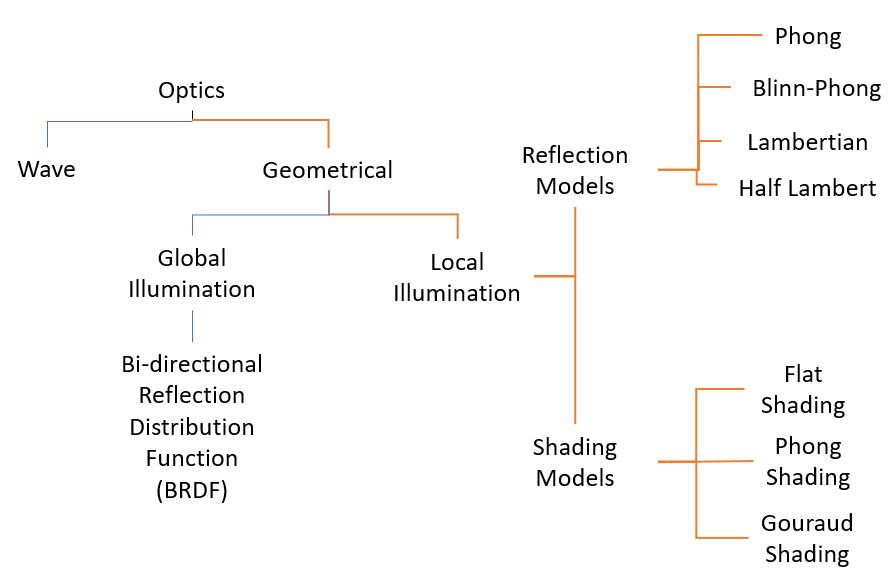
\includegraphics[scale=0.5]{./images/problem-domain-analysis}
	\caption{Problem Domain for Lighting Models of Computer Graphics.}
	\label{fig:prob-domain-analysis}
\end{figure}

The problem domain for lighting models in computer graphics is broad (Fig. 
\ref{fig:prob-domain-analysis}). To simplify this problem we invoke assumptions 
\aSref{geometrical_appx}, \aSref{illumination}, \aSref{illum_constraint}. This 
allows us to focus on the parts of the problem connected by the orange line.

The scope of the family includes geometrical optics simulation of light 
reflection for 3D material objects in a local illumination context.

\subsection{Characteristics of Intended Reader}
The intended readers of this document should have understanding of Grade 12 
Physics (particularly Optics) and a undergraduate Level 2 understanding of 
Linear Algebra and Matrix operations. 

\subsection{Organization of Document}
This document is organized in accordance with the CA template for scientific 
computing software provided by Dr. Smith for CAS 741. These templates are based 
on work by \citet{Smith2006}.

\section{General System Description}
This section identifies the interfaces between the system and its environment,
describes the potential user characteristics and lists the potential system
constraints.

\subsection{Potential System Contexts}
Figure \ref{fig:system-context} shows the high level system context. The circle 
represents the system user. The box is the library of lighting models system. 
Arrows are used to show the flow of data between the system and its environment.

\begin{figure}[h]
	\centering
	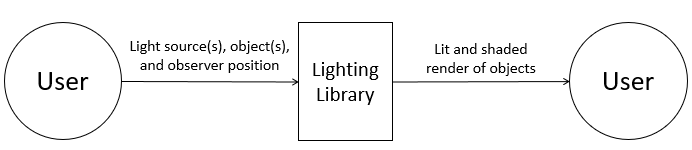
\includegraphics[scale=0.8]{./images/system-context}
	\caption{High level system context for \famname}
	\label{fig:system-context}
\end{figure}

\begin{itemize}
\item User Responsibilities:
\begin{itemize}
\item Ensure that problem they are looking to solve matches the assumptions 
made for this family.
\item Provide information on the light source(s), object(s) in scene, and 
observer position.
\item Declare shading model to use from preset options.
\item Declare lighting model to use from present options.
\item Ensure application programming interface use complies with the user guide.
\end{itemize}
\item \famname{} Responsibilities:
\begin{itemize}
\item Calculate the reflections of all light rays coming from the light 
source(s).
\item Determine which light rays (reflected or from source) reach the observer.
\item Render a lit environment based on selected shading and lighting model.
\item Update the calculations and render in response to changes in the input 
data.
\item Detect data type mismatch, such as a string of characters instead of a
  floating point number.
\end{itemize}
\end{itemize}

\subsection{Potential User Characteristics} \label{SecUserCharacteristics}

The end user of \famname{} should have an Computer Science/Software Engineering 
Undergraduate Level 3 understanding of Computer Graphics (such as through 
completing the SFWR ENG/CS 3GC3) and moderate experience with programming.

\subsection{Potential System Constraints}
There are no system constraints.

%\plt{You may not have any system constraints.}
%
%\plt{If you need to make design decisions for your family, these decisions will
%  be made here as constraints.  For instance, if all inputs will have to use 
%the
%same file format, this would be a constraint that would be included here.}
%
%\plt{You should generally limit the number of constraints, to keep the CA
%  abstract.}

\section{Commonalities}
This section presents a high-level view of the problem. It captures terminology 
and definitions relevant to the problem, theoretical models that are common to 
all members of the family, goal statements of the family, data definitions that 
will be used to solve these problems, as well as commonalities in inputs, 
calculations, and outputs.

This section also provides a background overview which explains the motivation 
for this work.

\subsection{Background Overview} \label{Sec_Background}

\subsection{Terminology and  Definitions}
This subsection provides a list of terms that are used in the subsequent
sections and their meaning, with the purpose of reducing ambiguity and making it
easier to correctly understand the requirements:

\begin{itemize}

\item Geometrical Optics: The study of lights as rays.
\item Reflection:
\item Specular reflection:
\item Diffuse reflection:
\item Refraction:
\item Lighting model:
\item Global illumination:
\item Emissive illumination:
\item Ambient light: Light with no identifiable source or direction.
\item Directional light: Light defined only by direction; light travels 
infinitely in that single direction.
\item Point light: Light defined only by a point; light travels uniformly in 
every direction from that point, with intensity decreasing with square of 
distance from source.
\item Spotlight: Light defined by a point and direction; light travels 
infinitely in a single direction from the defined source point.
\item Shading model:
\item OpenGL:

\end{itemize}

\subsection{Data Definitions} \label{sec_datadef}
This section collects and defines all the data needed to build the instance
models. The dimension of each quantity is also given.  \plt{Modify the examples
  below for your problem, and add additional definitions as appropriate.}

~\newline

\noindent
\begin{minipage}{\textwidth}
\renewcommand*{\arraystretch}{1.5}
\begin{tabular}{| p{\colAwidth} | p{\colBwidth}|}
\hline
\rowcolor[gray]{0.9}
Number& DD\refstepcounter{datadefnum}\thedatadefnum \label{FluxCoil}\\
\hline
Label& \bf Heat flux out of coil\\
\hline
Symbol &$q_C$\\
\hline
% Units& $Mt^{-3}$\\
% \hline
  SI Units & \si{\watt\per\square\metre}\\
  \hline
  Equation&$q_C(t) = h_C (T_C - T_W(t))$, over area $A_C$\\
  \hline
  Description & 
                $T_C$ is the temperature of the coil (\si{\celsius}).  $T_W$ is the temperature of the water (\si{\celsius}).  
                The heat flux out of the coil, $q_C$ (\si{\watt\per\square\metre}), is found by
                assuming that Newton's Law 
                of Cooling applies (\aref{A_Newt_coil}).  This law (\dref{NL}) is used on the surface of
                the coil, which has area $A_C$ (\si{\square\metre}) and heat 
                transfer coefficient $h_C$
                (\si{\watt\per\square\metre\per\celsius}).  This equation
                assumes that the temperature of the coil is constant over time (\aref{A_tcoil}) and that it does not vary along the length
                of the coil (\aref{A_tlcoil}).
  \\
  \hline
  Sources& Citation here\\
  \hline
  Ref.\ By & \iref{ewat}\\
  \hline
\end{tabular}
\end{minipage}\\

\subsection{Goal Statements}

\noindent Given some light source(s), some object(s) and their respective 
material properties, and an observer the goal statements are:

\begin{itemize}

\item[GS\refstepcounter{goalnum}\thegoalnum \label{display}:] 
Render a fully lit and shaded scene of the objects based on the observer 
location.
%\plt{One
%    sentence description of the goal.  There may be more than one.  Each Goal
%    should have a meaningful label.}

\end{itemize}

\subsection{Theoretical Models} \label{sec_theoretical}

This section focuses on the general equations and laws that \famname{} is based
on.  %\plt{Modify the examples below for your problem, and add additional models
%  as appropriate.}

~\newline

\noindent
\begin{minipage}{\textwidth}
\renewcommand*{\arraystretch}{1.5}
\begin{tabular}{| p{\colAwidth} | p{\colBwidth}|}
  \hline
  \rowcolor[gray]{0.9}
  Number& T\refstepcounter{theorynum}\thetheorynum \label{TM_Reflection}\\
  \hline
  Label&\bf Law of Reflection\\
  \hline
  Equation&   $\angle\theta_{i} = \angle\theta_{r}$ or $\hat{I}\bullet\hat{N} = 
  \hat{R}\bullet\hat{N}$\\
  \hline
  Description & 
                When a ray of light reflects off a surface, the angle of 
                incident is equal to the angle of reflection. This can also be 
                written as the dot product of the incident ray and the normal 
                is equal to the dot product of the reflected ray and the 
                normal.
		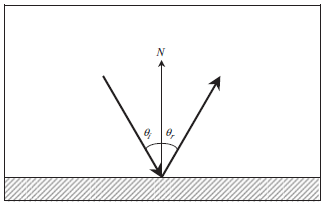
\includegraphics[scale=1]{./images/specular-reflection}  
		\\              
                                
  \hline
  Source &
           \url{}\\
  % The above web link should be replaced with a proper citation to a publication
  \hline
  Ref.\ By & \dref{ROCT}\\
  \hline
\end{tabular}
\end{minipage}\\

~\newline

%\plt{In a CA, the TMs often do not need to be refined.  However, this is not a
%  rule.  In some cases, it may make sense to introduce an IM, or possibly even 
%a
%  GD in between the TM and the IM.}

\subsubsection{General Definitions}\label{sec_gendef}

%\plt{General Definitions (GDs) are a refinement of one or more TMs, and/or of
%	other GDs.  The GDs are less abstract than the TMs.  Generally the reduction
%	in abstraction is possible through invoking (using/referencing) Assumptions.
%	For instance, the TM could be Newton's Law of Cooling stated abstracting.  
%	The GD could take the general law and apply it to get a 1D equation.}

This section collects the laws and equations that will be used in building the
instance models.

%\plt{Some projects may not have any content for this section, but the section
%	heading should be kept.}  \plt{Modify the examples below for your problem, 
%	and
%	add additional definitions as appropriate.}

~\newline

\noindent
\begin{minipage}{\textwidth}
	\renewcommand*{\arraystretch}{1.5}
	\begin{tabular}{| p{\colAwidth} | p{\colBwidth}|}
		\hline
		\rowcolor[gray]{0.9}
		Number& GD\refstepcounter{defnum}\thedefnum \label{diffReflect}\\
		\hline
		Label &\bf Diffuse Reflection \\
		\hline
		% Units&$MLt^{-3}T^0$\\
		% \hline
		SI Units& - \\
		\hline
		Equation& $ \angle\theta_{i} = \angle\theta_{r}$  \\
		\hline
		Description &
		Law of Reflection applied to rough surfaces.
		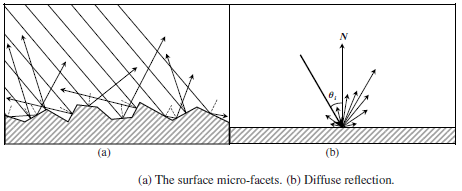
\includegraphics[scale=1]{./images/diffuse-reflection}
		\\
		\hline
		Source & Citation here \\
		\hline
		Ref.\ By & \ddref{FluxCoil}, \ddref{FluxPCM}\\
		\hline
	\end{tabular}
\end{minipage}\\

\section{Variabilities}
The follow section outlines variabilities between family members. Section 
\ref{sec_Assumptions} covers the assumptions made to simplify/realise the 
problem. Section \ref{sec_Calculation} captures variabilities in the 
implementation.

%\plt{The variabilities are summarized in the following subsections.  They may
%  each be summarized separately, like in \citet{SmithMcCutchanAndCarette2017}, 
%  or in a table, as in \citet{Smith2006}.}
%
%\plt{For each variability, a description should be given, along with the
%  parameters of variation and the binding time.  The parameters of variation
%  give the type that defines possible values.  The binding time is when the
%  variability is set.  The possible values are specification time (scope time),
%  build time and run time.}

Before tackling those sections, we summarize here variabilities in the problem.

\subsection{Assumptions} \label{sec_Assumptions}
This section outlines the various assumptions made in defining this problem. 
These assumptions are divided based on their binding time.

\begin{itemize}
	\item \textbf{Scope Time Bindings}:
	\begin{itemize}
		\item[AS\refstepcounter{assumpnumS}\theassumpnumS\label{geometrical_appx}:]
		Light will be defined by Geometrical Optics principles (ray-based).
		\item[AS\refstepcounter{assumpnumS}\theassumpnumS\label{illumination}:] 
		Lighting will be handled at the local illumination level.
		\item[AS\refstepcounter{assumpnumS}\theassumpnumS\label{illum_constraint}:]
		Objects will not reflect light at each other.
	\end{itemize}
	\item \textbf{Build Time Bindings}:
	\begin{itemize}
		\item[AB\refstepcounter{assumpnumB}\theassumpnumB\label{coordinates}:]
		Positions of light source(s), object(s), and the observer will be 
		defined on a 3D Cartesian Coordinate System.
		\item[AB\refstepcounter{assumpnumB}\theassumpnumB\label{object_representation}:]
		Objects will be represented by a geometric mesh of triangles.		
		\item[AB\refstepcounter{assumpnumB}\theassumpnumB\label{object_refraction}:]
		All objects are opaque; light will not experience refraction with any 
		object.			
	\end{itemize}
	\item \textbf{Run-Time Bindings}:
	\begin{itemize}
		\item[AR\refstepcounter{assumpnumR}\theassumpnumR\label{light_position}:]
		Position of light source will be defined by a vector $[x, y, z]$ 
		representing the Cartesian Coordinates of its centre.
		\item[AR\refstepcounter{assumpnumR}\theassumpnumR\label{light_type}:]
		Type of light source will be selected from the following list:
		\begin{enumerate}
			\item Point light,
			\item Spotlight,
			\item Directional light, or
			\item Ambient light.
		\end{enumerate}
		\item[AR\refstepcounter{assumpnumR}\theassumpnumR\label{light_colour}:]
		Colour of light from light source will be defined by a 3-tuple 
		$(r,g,b)$.
		\item[AR\refstepcounter{assumpnumR}\theassumpnumR\label{object_position}:]
		Position of light source will be defined by a vector $[x, y, z]$ 
		representing the Cartesian Coordinates of its centre.
		\item[AR\refstepcounter{assumpnumR}\theassumpnumR\label{object_type}:]
		Type of light source will be selected from the following list:
		\begin{enumerate}
			\item Sphere,
			\item Cube,
			\item Torus, or
			\item Teapot.
		\end{enumerate}
		\item[AR\refstepcounter{assumpnumR}\theassumpnumR\label{object_colour}:]
		Object material colour is defined by a 3-tuple $(r,g,b)$.				
	\end{itemize}	
\end{itemize}

Other assumptions about the system include:
\begin{itemize}
\item[A\refstepcounter{assumpnum}\theassumpnum \label{coordinate_system}:] The 
virtual environment will be described by a 3D Caretsian Coordinate System using 
right-hand rules.
\item[A\refstepcounter{assumpnum}\theassumpnum \label{light_source_input}:] 
Light source(s) information (position, type, colour) will be passed in via file.
\item[A\refstepcounter{assumpnum}\theassumpnum \label{object_input}:] 
Object(s) information (position, mesh, colour, material properties) will be 
passed in via file.
%  \plt{Short description of each assumption.  Each assumption
%    should have a meaningful label.  Use cross-references to identify the
%    appropriate traceability to T, GD, DD etc., using commands like dref, 
%ddref etc.}

\end{itemize}

%\plt{Input assumptions will be appropriate for many problems.  Some input will
%  have simplifying constraints, and other inputs will not.}

\subsection{Calculation} \label{sec_Calculation}

\begin{itemize}
	\item Abstract Variabilities:
	\begin{itemize}
		\item Position of the light sources.
		\item Position of the object(s)
	\end{itemize}
	\item Data Structure Variabilities:
	\begin{itemize}
		\item
	\end{itemize}
	\item Algorithmic Variabilities:
	\begin{itemize}
		\item Reflection model (how the reflections are calculated/realised)
		\item Shading model (Interpolation technique)
	\end{itemize}
\end{itemize}
%\plt{The calculation variabilities should be as abstract as possible.  If there
%  are variabilities that are related to imposed design decisions, the system
%  constraints section should be referenced for the relevant constraint.  Design
%  constraint related variabilities should be listed separately.}
%
%\plt{Variabilities related to data structure choices would go in this section.
%  However, these variabilities are related to design, so they should be
%  separated from the more abstract variabilities.}
%
%\plt{Algorithmic variations would go here as well, but as for data structures,
%  they should be separated from the more abstract variabilities.}

\subsection{Output} \label{sec_Output}    

\section{Requirements}

This section provides the functional requirements, the business tasks that the
software is expected to complete, and the nonfunctional requirements, the
qualities that the software is expected to exhibit.

\subsection{Family of Functional Requirements}

\plt{Since the CA will often be applied to a library, the functionality will not
  be a single use case.  Therefore, this section should summarize the family of
  potential requirements.  A good way to provide an overview of the functional
  requirements would be to provide multiple use cases on how the library will be
  employed.}

\noindent \begin{itemize}

\item[R\refstepcounter{reqnum}\thereqnum \label{R_Inputs}:] \plt{Requirements
    for the inputs that are supplied by the user.  This information has to be
    explicit.}

\item[R\refstepcounter{reqnum}\thereqnum \label{R_OutputInputs}:] \plt{It isn't
    always required, but often echoing the inputs as part of the output is a
    good idea.}

\item[R\refstepcounter{reqnum}\thereqnum \label{R_Calculate}:] \plt{Calculation
    related requirements.}

\item[R\refstepcounter{reqnum}\thereqnum \label{R_VerifyOutput}:]
  \plt{Verification related requirements.}

\item[R\refstepcounter{reqnum}\thereqnum \label{R_Output}:] \plt{Output related
    requirements.}

\end{itemize}

\subsection{Nonfunctional Requirements}

\plt{To allow the Non-Functional Requirements (NFRs) to vary between family
  members, try to parameterize them.  The value of the parameter is than a variability.}

\plt{An important variability between family members it the relative importance
  of the NFRs.  \citet{Smith2006} shows how pairwise comparisons can be used to
  rank the importance of NFRs.}

\plt{List your nonfunctional requirements.  You may consider using a fit
  criterion to make them verifiable.}

\section{Likely Changes}    

\noindent \begin{itemize}

\item[LC\refstepcounter{lcnum}\thelcnum\label{LC_refraction}:] Refractive 
materials incorporated into family.


\end{itemize}

\section{Traceability Matrices and Graphs}

\plt{You will have to add tables.}

\newpage

\bibliographystyle {plainnat}
\bibliography {../refs/References}

\newpage

\section{Appendix}

\plt{Your report may require an appendix.  For instance, this is a good point to
show the values of the symbolic parameters introduced in the report.}

\subsection{Symbolic Parameters}

\plt{The definition of the requirements will likely call for SYMBOLIC\_CONSTANTS.
Their values are defined in this section for easy maintenance.}

\noindent \plt{Advice on using the template:
\begin{itemize}
\item Assumptions have to be invoked somewhere
\item ``Referenced by'' implies that there is an explicit reference
\item Think of traceability matrix, list of assumption invocations and list of
  reference by fields as automatically generatable
\item If you say the format of the output (plot, table etc), then your
  requirement could be more abstract
\item For families the notion of binding time should be introduced
\item Think of families as a library, not as a single program
\end{itemize}
}

\end{document}